\label{evaluation}
\section{Experimental Results - Evaluation}
We run our web crawler described in section \ref{implementation} over the 100,000 most visited web sites as
rated by alexa.com.  The crawler uses heuristics in order to determine the type of defense a web site employs and
we provide no formal proof that our results are correct.  In this section we present our findings, regarding the
number of web sites that choose to use each defense.  In the rest of this section we evaluate the method we
used to conduct the experiment (our web crawler), compared to a very small number of web sites we examined manually. 

\subsection{Platform} 
We run our experiments on two Intel(R) Xeon(R) CPU E5405 with 8 cores @2.00GHz machines each with 12GB of RAM. 
One machine was running Red Hat Enterprise Linux Server 5.2 and the other CentOS 5.6. 
On each machine we raised 64 threads, since the greater portion of the time was spent on waiting 
for the requests to be served, the 8 cores could efficiently serve this number of threads.  Each machine used a list 
of 50,000 URLs we got from Alexa's Top 100,000 website list.  

\subsection{Results}
\begin{figure}[htb]
	%\centering
	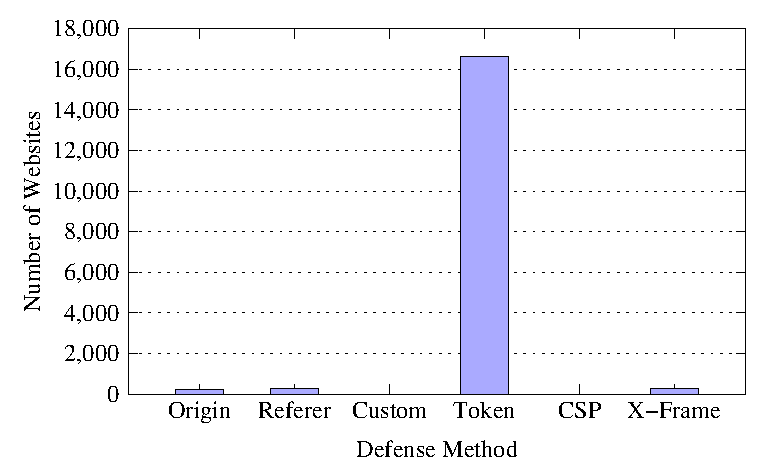
\includegraphics[scale=0.7]{figs/results_all}
	\caption{Prefered CSRF Defense Method for the 100,000 most visited websites}
	\label{fig:resultsAll}
\end{figure}

\begin{figure}[htb]
	%\centering
	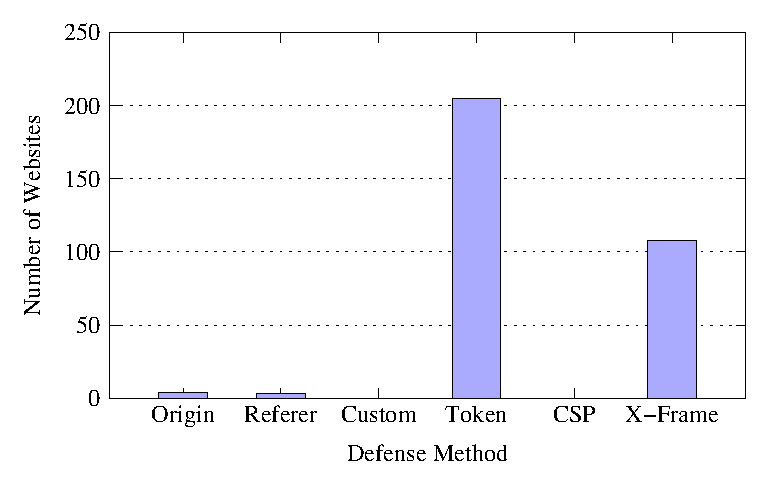
\includegraphics[scale=0.7]{figs/results_top}
	\caption{Prefered CSRF Defense Method for the 1,000 most visited websites}
	\label{fig:resultsTop}
\end{figure}

\begin{figure}
	\centering
		\begin{tabular}{|l|l|}
			\hline
			\multicolumn{2}{|c|}{Top 100,000 Websites} \\
			\hline
			Origin header & 221 \\
			\hline
			Referer header & 285 \\
			\hline
			Custom XMLHtmlHeader & 0 \\
			\hline
			Secret Token & 16633 \\
			\hline
			Content Security Policy header & 5 \\
			\hline
			X-Frame header & 260 \\
			\hline
	\end{tabular}
	\caption{Prefered CSRF Defense Method for the 100,000 most visited websites in absolute values}
	\label{table:resultsAll}
\end{figure}

\begin{figure}
	\centering
	\begin{tabular}{|l|l|}
			\hline
			\multicolumn{2}{|c|}{Top 1,000 Websites} \\
			\hline
			Origin header & 4 \\
			\hline
			Referer header & 3 \\
			\hline
			Custom XMLHtmlHeader & 0 \\
			\hline
			Secret Token & 205 \\
			\hline
			Content Security Policy header & 0 \\
			\hline
			X-Frame header & 108 \\
			\hline
	\end{tabular}
	\caption{Prefered CSRF Defense Method for the 1,000 most visited websites in absolute values}
	\label{table:resultsTop}
\end{figure}

Figure \ref{fig:resultsAll} shows the total number of websites that use each defense discussed in section \ref{defenses}. 
Origin bar refers to Origin header, Referer bar to Referer header, Custom to Custom XMLHtmlHeader, Token to Secret Validation
Token, X-Frame to X-Frame header and CSP to Content Security Policy header.  
We see that the preferred method by far, according to our tool's judgement, is the use of secret validation tokens in submit Forms.  
We also notice that the Referer and Origin Headers appear to be used in equal frequency.  Another point of interest is that we did not detect any 
custom XMLHtmlHeaders, which is an unexpected result.  We did not manage to see whether this is accurate or an implementation bug, note
that we did, indeed, not find any such headers in the websites we manually examined.  Moreover, the Contet-Security-Policy appears in some
rare cases and only in websites that hold high places in alexa's list, while the X-Frame header is used much more frequently.  Although,
the X-Frame offers only a subset of the Content Security Policy's functionalities (namely restricting content to be loaded in frames), the
later is a relative new header and has just been implemented in major web browsers, while the X-Frame header has been around for a much
longer period.  We expect that more websites will start using the Content Security Policy header in the near future.

Figures \ref{fig:resultsTop} and \ref{table:resultsTop} show the preferred defense method for the first 1,000 most visited websites, as found in
alexa.com index.  The results draw a similar picture to those in shown in \ref{fig:resultsAll} and \ref{table:resultsAll}. 

\subsection{Method Evaluation}
Our method use heuristics in order to associate a defense mechanism with a web site.  This leaves a big margin
for error which renders it difficult to prove the correctness of our results.  Parsing the header to determine the
different header fields is trivial, but determining if a web site uses secret tokens is not, for two main reasons.
\begin{enumerate}
 \item The vast set of possible token values, makes it hard, if not unfeasible to formalize a way to determine 
 is an arbitrary string value is a token value.  On many cases, the token is a hash value, but this not the 
 necessarily true for all tokens
 \item Using secret tokens to protect forms, is crucial when the user has already been authorized.  It 
 is unrealistic for our crawler to get authorized access to all web sites, and then parse its content
\end{enumerate} 
We present two cases, where our method failed or was partially correct.  The first case is paypal, which protects none
of its forms with any token, even the login form when an unauthorized user is viewing the website.  When a user is granted
authorization, we found out that the forms contained a hidden Input field with a secret token.  The second case, is 
facebook, where the login form is originally protected by a token, that is generated using the current timestamp.  This
does not offer the desired security for an authorized user, thus when a user logs in, facebook generates a second 
token, which is session depended.  Furthermore, we provide the number of false positives we found by manually examining 
the first 100 websites on alexa's list. Out of 22 possible tokens found only 7 were actually token values, which gives us 
a false possitive percentage of 68\%.  Unfortunatelly, we are not able to provide a less intuitive metric regarding our tool's
performance ability to find secret token values.

